\section{Metodología}
Se entiende por Inteligencia Artificial a una simulación de procesos computacionales cognitivos para que simulen el comportamiento de una mente humana, estos comportamientos abarcan diferentes áreas de investigación, como el aprendizaje, comunicación, percepción, razonamiento y la capacidad de desarrollarse en entornos más complejos.

\subsection{Red neuronal}
Una red neuronal es una herramienta derivada de la inteligencia artificial que utiliza modelos matemáticos para ser utilizada como un mecanismo de predicción del texto. Son una forma de hacer que las computadoras aprendan, donde la computadora aprende a realizar alguna tarea analizando ejemplos de entrenamiento. Por lo general, estos ejemplos han sido etiquetados previamente.\\\\
Las redes neuronales son modeladas vagamente asemejando el cerebro humano, esta consiste en miles de millones de nodos que realizan el procesamiento de la información los cuales están densamente interconectados.\\\\
La complejidad de las neuronas reales se abstrae mucho cuando se realiza el modelado de neuronas artificiales. Estas consisten básicamente en entradas, que se multiplican por pesos (fuerza de las respectivas señales), y luego calculada por una función matemática que determina la activación de la neurona. Otra función (que puede ser la de identidad) calcula la salida de la neurona artificial (a veces en dependencia de un cierto umbral). Las redes neuronales combinan neuronas artificiales para procesar información.\cite{neuronart}

\begin{figure}[h]
	\centering
	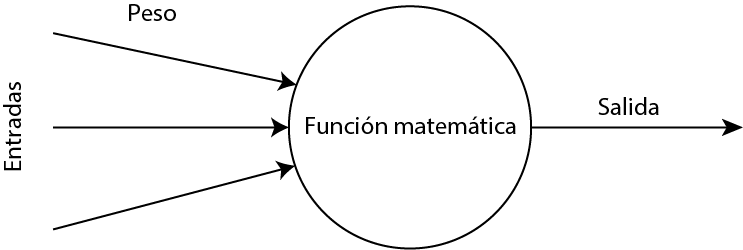
\includegraphics[width=8cm]{figuras/NeuronaArt.png}
	\caption{Neurona artificial.}
	\label{fig:Neurona artificial}
\end{figure}

\subsection{Recurrent Neural Network (RNN) – Long Short Term Memory (LSTM)}
Una red neuronal recurrente es un tipo de red neuronal artificial donde la salida de alguna capa en particular es salvada y sirve para retroalimentar la entrada de esta capa, lo cual ayuda a predecir futuras salidas de esta.
\begin{figure}[h]
	\centering
	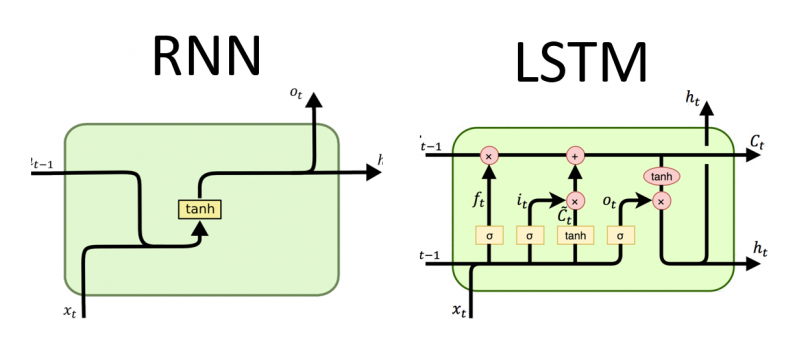
\includegraphics[width=8cm]{figuras/RnnLstm.png}
	\caption{Diagrama de las redes neuronales RNN y LSTM.}
	\label{fig:Diagrama de las redes neuronales RNN y LSTM}
\end{figure}
La primera capa está formada de la misma manera que la Feed-forward Neural Network, es decir, solo pasa la información que entra a la siguiente capa inmediata, posteriormente la siguiente capa con el paso del tiempo comenzará a retroalimentarse, pero manteniendo la propagación frontal. Haciendo uso de esta retroalimentación la capa en futuras operaciones puede realizar predicciones, si estas predicciones no son los resultados esperados, el sistema aprende y trabaja para corregir sus futuras predicciones.\cite{redneurnn}\\\\
Este tipo de redes neuronales se distinguen por su “memoria”, ya que toman información de entradas anteriores para influir en la entrada y salida actuales.

\subsection{Obtención del conjunto de datos}
El primer paso para poder empezar a trabajar con nuestro modelo fue obtener un conjunto de datos que cumpliera con las características que se necesitaban, por eso nos dimos a la tarea de buscar uno. En Kaggle \cite{kaggle1} se encontró un dataset llamado “Song lyrics for 6 musical genres” \cite{kaggleDataset} el cual contenía los datos necesarios y contaba con un total de 160,790 letras, las cuales pertenecían a 6 tipos de géneros musicales:
\begin{itemize}
	\item Rock
	\item Pop
	\item Hip Hop
	\item Samba
	\item Sertanejo
	\item Funk Carioca
\end{itemize}
Debido a que estas letras de canciones pertenecían a distintos géneros e idiomas se procedió a realizar una limpieza a la base de datos para quedarnos únicamente con las letras de canciones pertenecientes al genero pop y que estuvieran en el idioma inglés, además haciendo uso de la librería de “Pandas” y siguiendo el estándar de limpieza de datos: \cite{data_cleaning}
\begin{enumerate}
	\item Remover caracteres innecesarios
	\item Eliminar Duplicados
	\item Evitar errores ortográficos de similitud
	\item Convertir los tipos de dato
	\item Tratar los valores nulos o faltantes
\end{enumerate}
Se obtuvo como resultado un conjunto de datos útil, el cual solo cuenta con los datos necesarios para después poder tratarlos y utilizarlos para empezar el entrenamiento del modelo de la red neuronal, cabe destacar que este proceso es necesario hacerlo solo una vez para cada género musical ingresado, en caso de que se lleguen a necesitar más datos, será necesario repetir el proceso.
\subsection{Modelo}
Para el desarrollo del modelo se utilizó una libreta de Kaggle. Cabe mencionar que el lenguaje de programación utilizado para el desarrollo del modelo fue Python, por ende, lo primero que se trabajó en la libreta, fue realizar la importación de librerías que se fueran a necesitar, en este caso las más importantes son:
\begin{itemize}
	\item Pandas: la cual nos permite manipular y analizar la información.
	\item Wordcloud: es una herramienta que nos ayuda al momento de generar la siguiente palabra de una oración.
	\item Tensorflow: una herramienta que nos ayuda en el procesamiento del aprendizaje automático.
	\item Keras: una herramienta que nos ayuda en el procesamiento del aprendizaje profundo.
\end{itemize}
A continuación, procedemos a importar el conjunto de datos previamente trabajado y limpiado, pero en esta ocasión apoyándonos de la librería de pandas, solo nos vamos a quedar con letra de estas canciones, ya que es la información que nos interesa trabajar y la cual vamos a estar manipulando.\\\\
Al usar Kaggle debemos tener en cuenta sus limitantes, en este caso se cuenta solamente con 16Gb de RAM, un disco de 73Gb y una GPU de 13GB para el procesamiento de nuestro conjunto de datos, por eso debemos limitar nuestro modelo, en lugar de utilizar todos los datos (28441), vamos a trabajar solo con 700 letras de canciones por el momento.\\\\ 
Utilizando estas 700 lyrics, se decidió obtener información de ellas, siendo más específicos, estadísticas sobre el número de palabras en cada canción, esto con el fin de determinar la frecuencia de distribución del número de palabras de cada texto y para tener una idea del promedio de palabras, esto con el fin de tenerlo en cuenta al momento de realizar la generación de texto.
\begin{figure}[h]
	\centering
	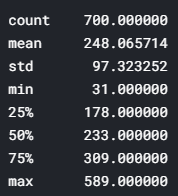
\includegraphics[width=4cm]{figuras/estadistica.png}
	\caption{Estadisticas de las palabras}
	\label{fig:Estadisticas_de_las_palabras}
\end{figure}
Lo que podemos observar en la imagen anterior es:
\begin{itemize}
	\item Count: el cual es el número de canciones analizadas.
	\item Mean: el promedio de palabras por canción.
	\item Std: la desviación estándar de las palabras.
	\item Min: la menor cantidad de palabras encontradas en una canción.
	\item Max: la mayor cantidad de palabras encontradas en una canción.
\end{itemize}
Además, se le realizo una tokenizacion a las letras de nuestras 700 canciones, esto quiere decir que se separó cada palabra y cada palabra se convirtió en un número. Para este proceso se hizo uso de Keras y la clase Tokenizer().
\begin{figure}[h]
	\centering
	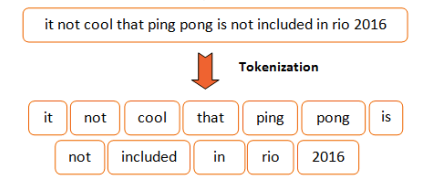
\includegraphics[width=8cm]{figuras/tokenization.png}
	\caption{Tokenizado de las palabras \cite{tokenimagen}}
	\label{fig:Tokenizado de las palabras}
\end{figure}
Antes de la generación del modelo, es necesario normalizar todas las oraciones a una misma longitud estándar, para evitar el desbordamiento de la memoria y conseguir que las capas del modelo sean mucho más profundas, este es un proceso simple el cual consta de agregar ceros al comienzo del texto, dando como resultado capas del mismo tamaño, a este proceso se le conoce como padding.\\\\
La posición donde se sumarán los ceros viene determinada por el relleno del argumento, en este caso, se hará al comienzo de la secuencia.
\begin{figure}[h]
	\centering
	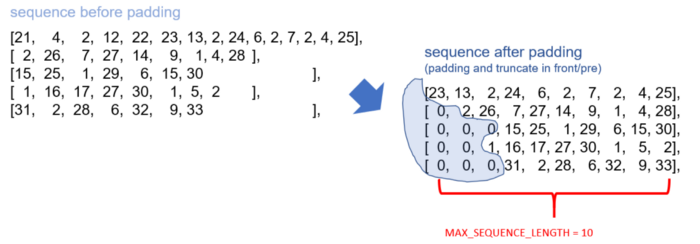
\includegraphics[width=8cm]{figuras/padding.png}
	\caption{Padding del tokenizado de las palabras}
	\label{fig:Padding del tokenizado de las palabras}
\end{figure}
\subsection{Creación del modelo}
En este caso se utilizó el modelo LSTM Bidireccional, este tipo de redes neuronales se ejecutan como su nombre lo indica: en dos direcciones. Esto quiere decir que va del pasado al futuro y viceversa, así es como el modelo conserva la información de ambos estados en cualquier momento. Las redes neuronales de LSTM se utilizan principalmente cuando el contexto está involucrado.\\\\
Los modelos en Keras se definen como una secuencia de capas, y el modelo secuencial se trata de agregar capas de una en una. Las capas son el componente básico de la red neuronal.\\\\
Dentro de estas capas podemos encontrar:
\subsubsection{Embedding o incrustación}
Es una capa central, solo se puede usar como la primera capa en un modelo, convierte los números enteros positivos en vectores densos de un tamaño fijo (el primer parámetro es el tamaño del vocabulario, el segundo parámetro es la dimensión de la incrustación densa y el tercer parámetro es sobre la longitud de las secuencias, este se requiere ya que usaremos una capa densa más adelante)
\subsubsection{Bidireccional}
Es una capa recurrente, una envoltura bidireccional para las redes neuronales de tipo RNN's que recibirá una capa como entrada, siendo la capa LSTM la que elegimos, recibirá un entero positivo como entrada que se refiere a la cantidad de nodos de salida que se deben devolver.
\subsubsection{Dropout}
Es una capa de regularización. Esta capa establece aleatoriamente las unidades de entrada en 0, con una frecuencia del valor que le pasamos, en cada paso durante el tiempo de entrenamiento, lo que ayuda a evitar el sobreajuste.
\subsubsection{Densidad}
Es una capa central y una capa de red neuronal densamente conectada. Recibe como primer parámetro un entero positivo que se refiere a la cantidad de nodos de salida que deben devolverse. El segundo parámetro es el llamado activación que define el tipo de predicciones que puede hacer el modelo; para el tipo de problema que estamos considerando, el que se adapta mejor es softmax, que genera un vector de valores (entrada) que puede interpretarse como probabilidades de ser utilizado.
\subsubsection{Método de compilación, algoritmo de optimización y métrica de rendimiento}
Perdida: También conocida como función de costos; funciona durante el proceso de optimización y su función es calcular el error del modelo. La entropía cruzada se utiliza para estimar la diferencia entre una distribución de probabilidad estimada y predicha. Se utilizará categorical\_cross-entropy porque es más adecuado para este tipo de problemas y se usa casi universalmente para entrenar redes neuronales de aprendizaje profundo debido a los resultados que produce.\\\\
Optimización: Se encarga de reducir las pérdidas y brindar los resultados más precisos posibles. Adam es la opción elegida porque es la mejor opción que ofrece Keras para entrenar la red neuronal en menos tiempo y de manera más eficiente. Earlystop detendrá el entrenamiento si el modelo ha dejado de mejorar, esto se verificará al final de cada epoch. En este caso, la "precisión" o “accuracy” se utilizará como métrica de rendimiento.
El método fit es el encargado de entrenar el modelo para el número fijo de epochs dados.\\\\
Quedando como resultado el código del modelo de la siguiente forma:

\begin{center}
	\lstinputlisting[language=Python]{figuras/modelo.py}
\end{center}
\subsubsection{Importación del modelo y función de generación}
Una vez completado el entrenamiento de nuestro modelo, lo que falta es importarlo para probar cómo funciona, en nuestro caso nombramos al modelo “song\_lyrics\_generator” y se importó de la siguiente forma:

\begin{center}
	\lstinputlisting[language=Python]{figuras/import.py}
\end{center}
Ya que contemos con el modelo importado, se creó una función que se utilizará para generar la letra de una canción utilizando el modelo previamente entrenado, predecirá las siguientes palabras en base a la palabra(s) de entrada suministradas como 'seed\_text'. Para que esto funcione, se debe aplicar una tokenización al seed\_text, luego se aplicará un relleno a las secuencias generadas y se pasará al modelo entrenado para que se pueda predecir la siguiente palabra.

\begin{center}
	\lstinputlisting[language=Python]{figuras/function.py}
\end{center}
